% !Mode:: "TeX:UTF-8"

\chapter{系统整体设计}[overall]
\label{chapter:overall}

本章简明描述本文所设计的操作系统的体系结构和主要的构成模块,旨在对整个操作系统有一个整体的把握。目前暂时将这个操作系统命名为“Moonix”,后文中的“Moonix”皆指本文所设计实现的操作系统。

目前,整个Moonix操作系统设计有两个部分组成:监管者模式部分和用户模式部分。监管者模式部分即操作系统内核,用于对硬件资源进行抽象和调度访问,向下沟通位于机器模式的SBI,向上应答用户模式的服务请求。用户模式部分,即操作系统服务,目前主要实现的是内核编程接口,用户编写的程序不会直接向监管者模式请求服务,而是通过调用内核编程接口函数,由这些函数代为请求。

Moonix整体采用了宏内核模式。宏内核的优点是执行速度快,缺点则是层次结构性不强。尽管如此,我们还是可以将其大概划分为以下四个模块:中断处理模块、内存管理模块、进程调度模块和文件系统模块。从宏内核模式结构模型(分层思想)出发,我们可以将Moonix的层次结构大致描述为图 \ref{pic:moonixtotal}。

\begin{figure}[htpb]
	\centering
	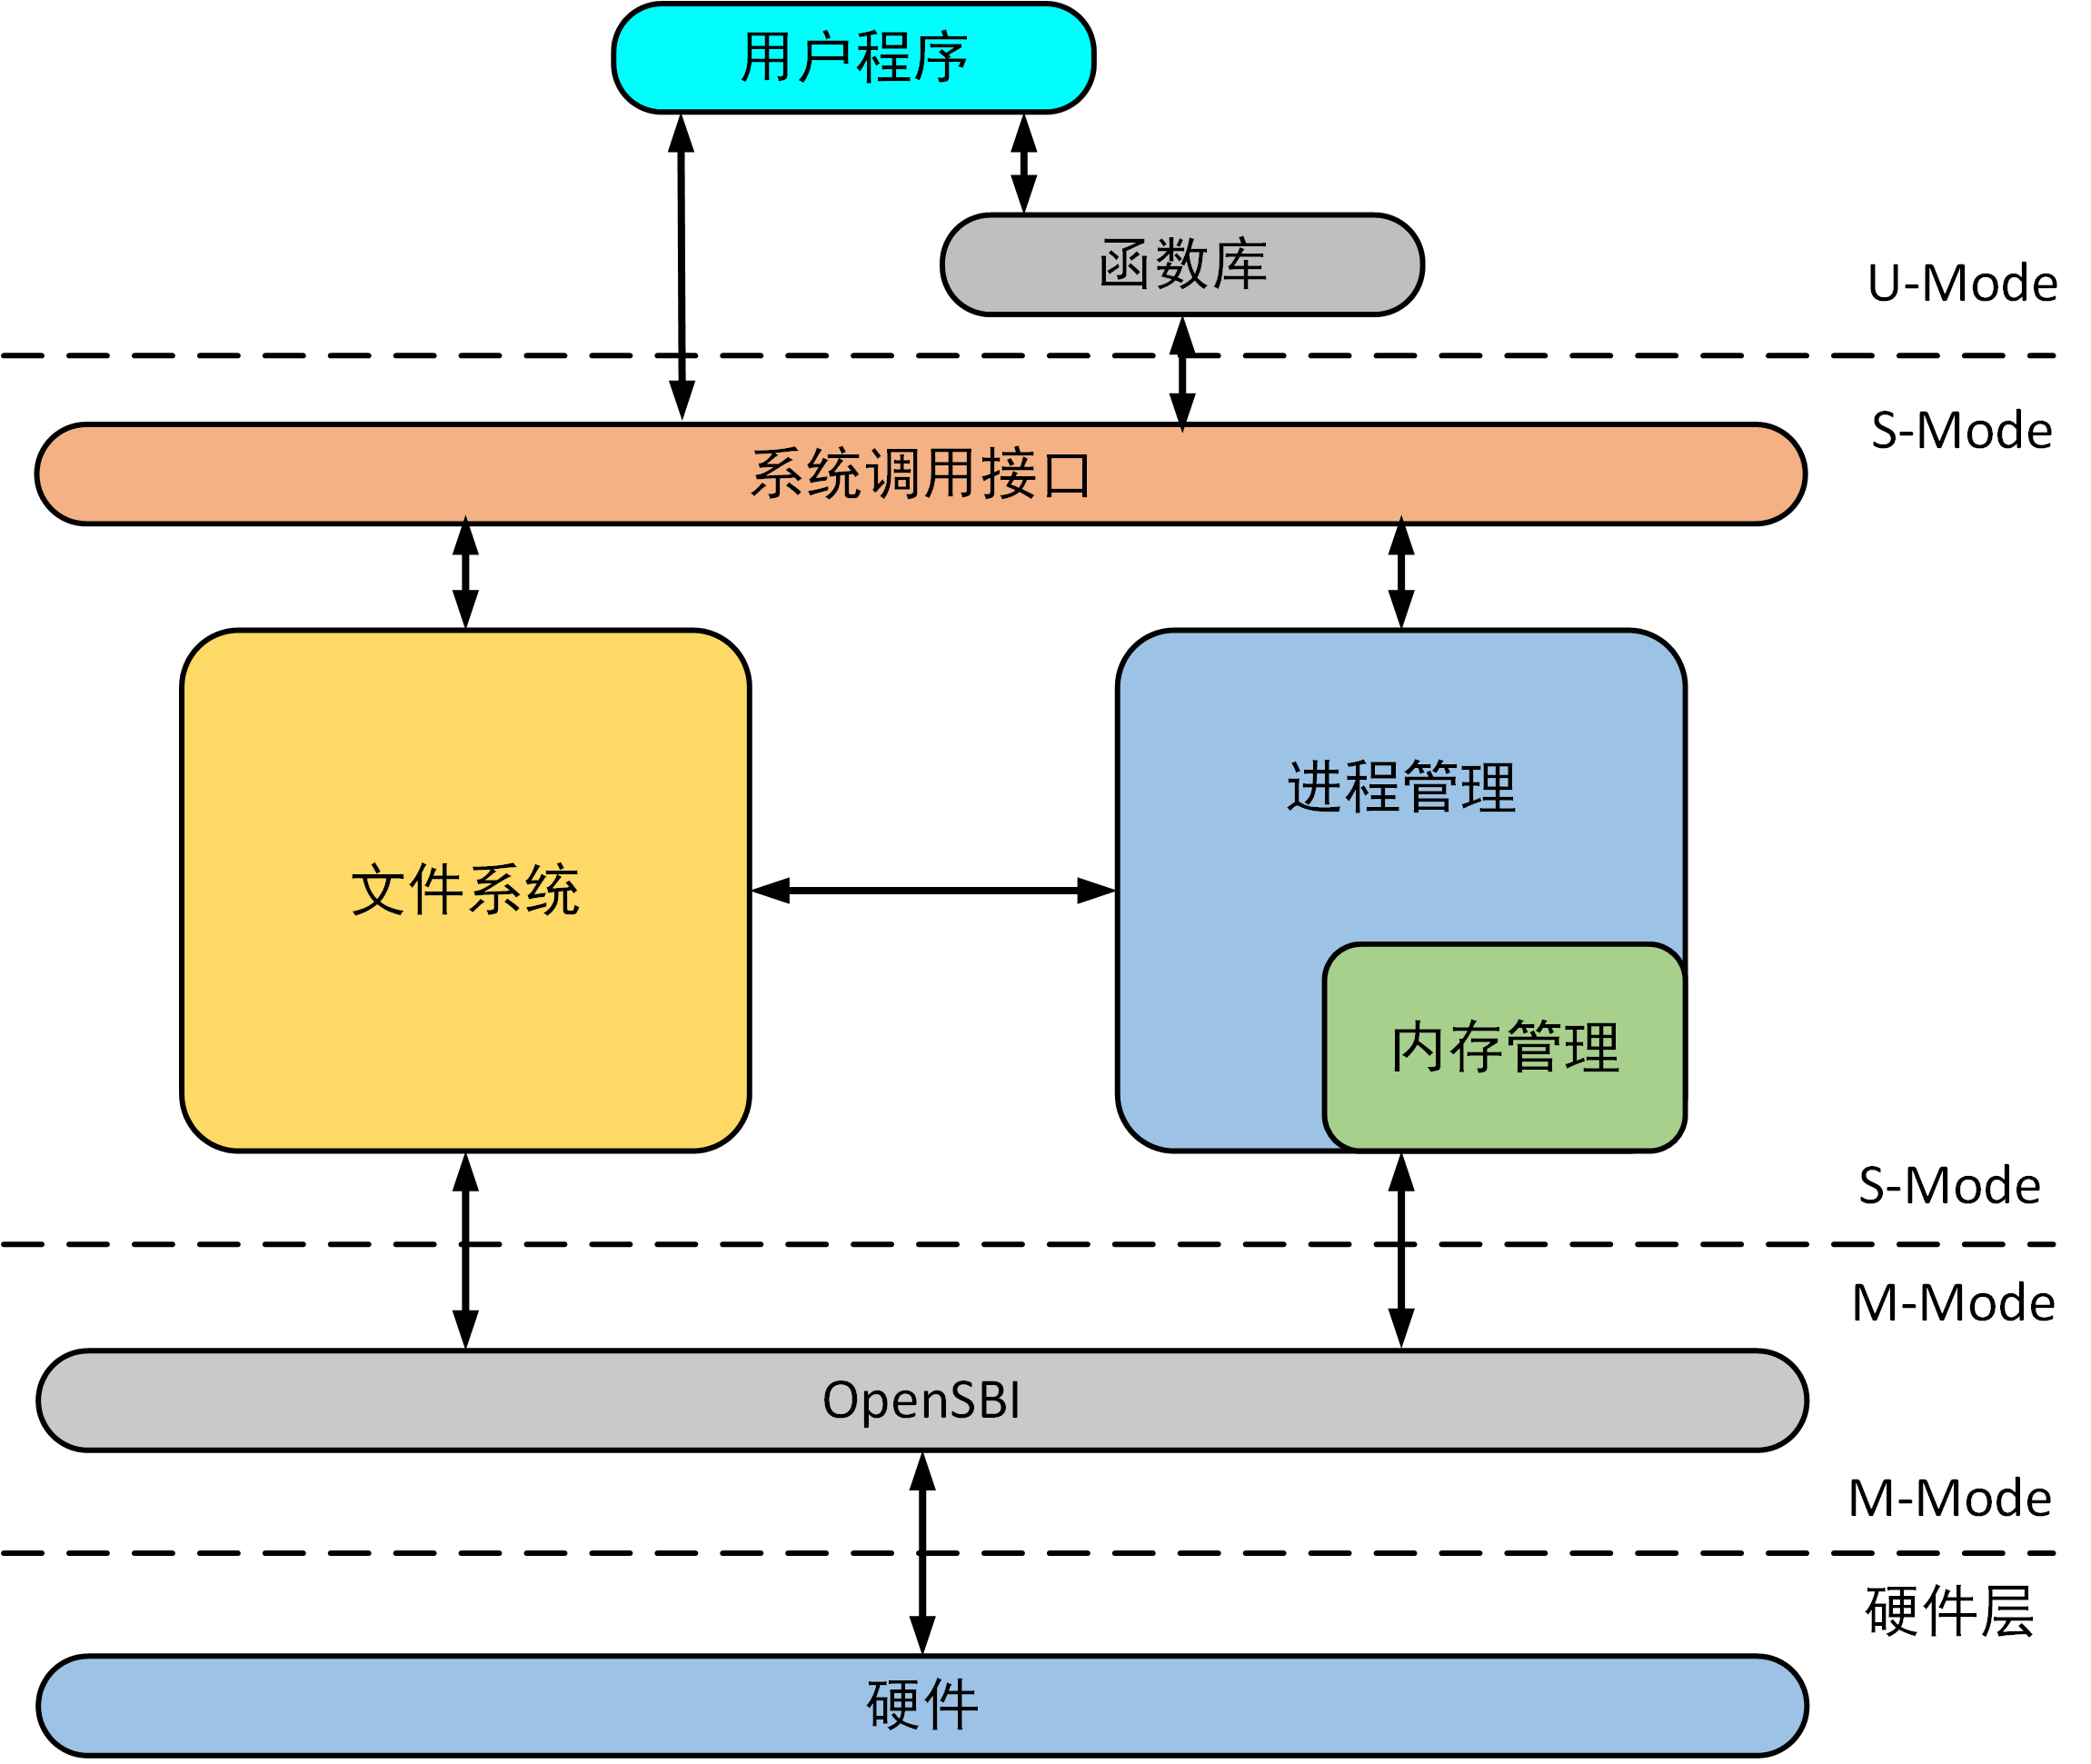
\includegraphics[width=0.55\textwidth]{moonixtotal}
	\setlength{\abovecaptionskip}{2pt}
	\caption{Moonix体系结构}
	\label{pic:moonixtotal}
\end{figure}

中断处理模块用于控制操作系统对内外部中断的响应。操作系统通过响应定时器中断,来定时检查进程的运行状态,可以说中断处理是进程调度的基础。内存管理模块主要通过虚拟内存管理的方式,保证各个进程能够安全共享物理内存,互不干扰。同时,由于各个进程都运行在独立的虚拟内存空间,使得各个程序实现时不必考虑实际的物理内存状态,降低了应用程序的实现难度。进程调度模块用来控制进程对CPU的使用,通过Round-Robin算法\cite{DBLP:journals/eor/RasmussenT08},来保证各个进程能够公平地使用CPU资源,同时内核也能够及时地响应外部中断。文件系统模块屏蔽了不同文件系统的细节,提供了一个通用的文件接口,供操作系统获取文件资源。

Moonix操作系统目前只能运行在QEMU虚拟机模拟的virt计算机上,以OpenSBI作为SBI。因此,Moonix可管理的内存受制于virt和OpenSBI。整个virt计算机可用物理内存大小为128MB,除去OpenSBI和Moonix内核占据的内存外,其余的内存都是Moonix操作系统可以管理的内存区域。

Moonix采用RISC-V指令集架构提供的Sv39系统来对内存进行虚拟化管理。Moonix将全部的128MB物理内存映射到一个512GB大小的虚拟地址空间中,并通过填充页表来对这种映射关系进行管理,CPU在进行地址解析时就可以通过页表来执行自动的地址翻译。在Moonix中,不同的进程可以拥有不同的页表,这意味着它们运行在相互隔离的虚拟地址空间中。当一个用户进程在运行时,虚拟地址空间和虚拟地址空间的布局和映射关系如图 \ref{pic:moonixmem} 所示。

\begin{figure}[htpb]
	\centering
	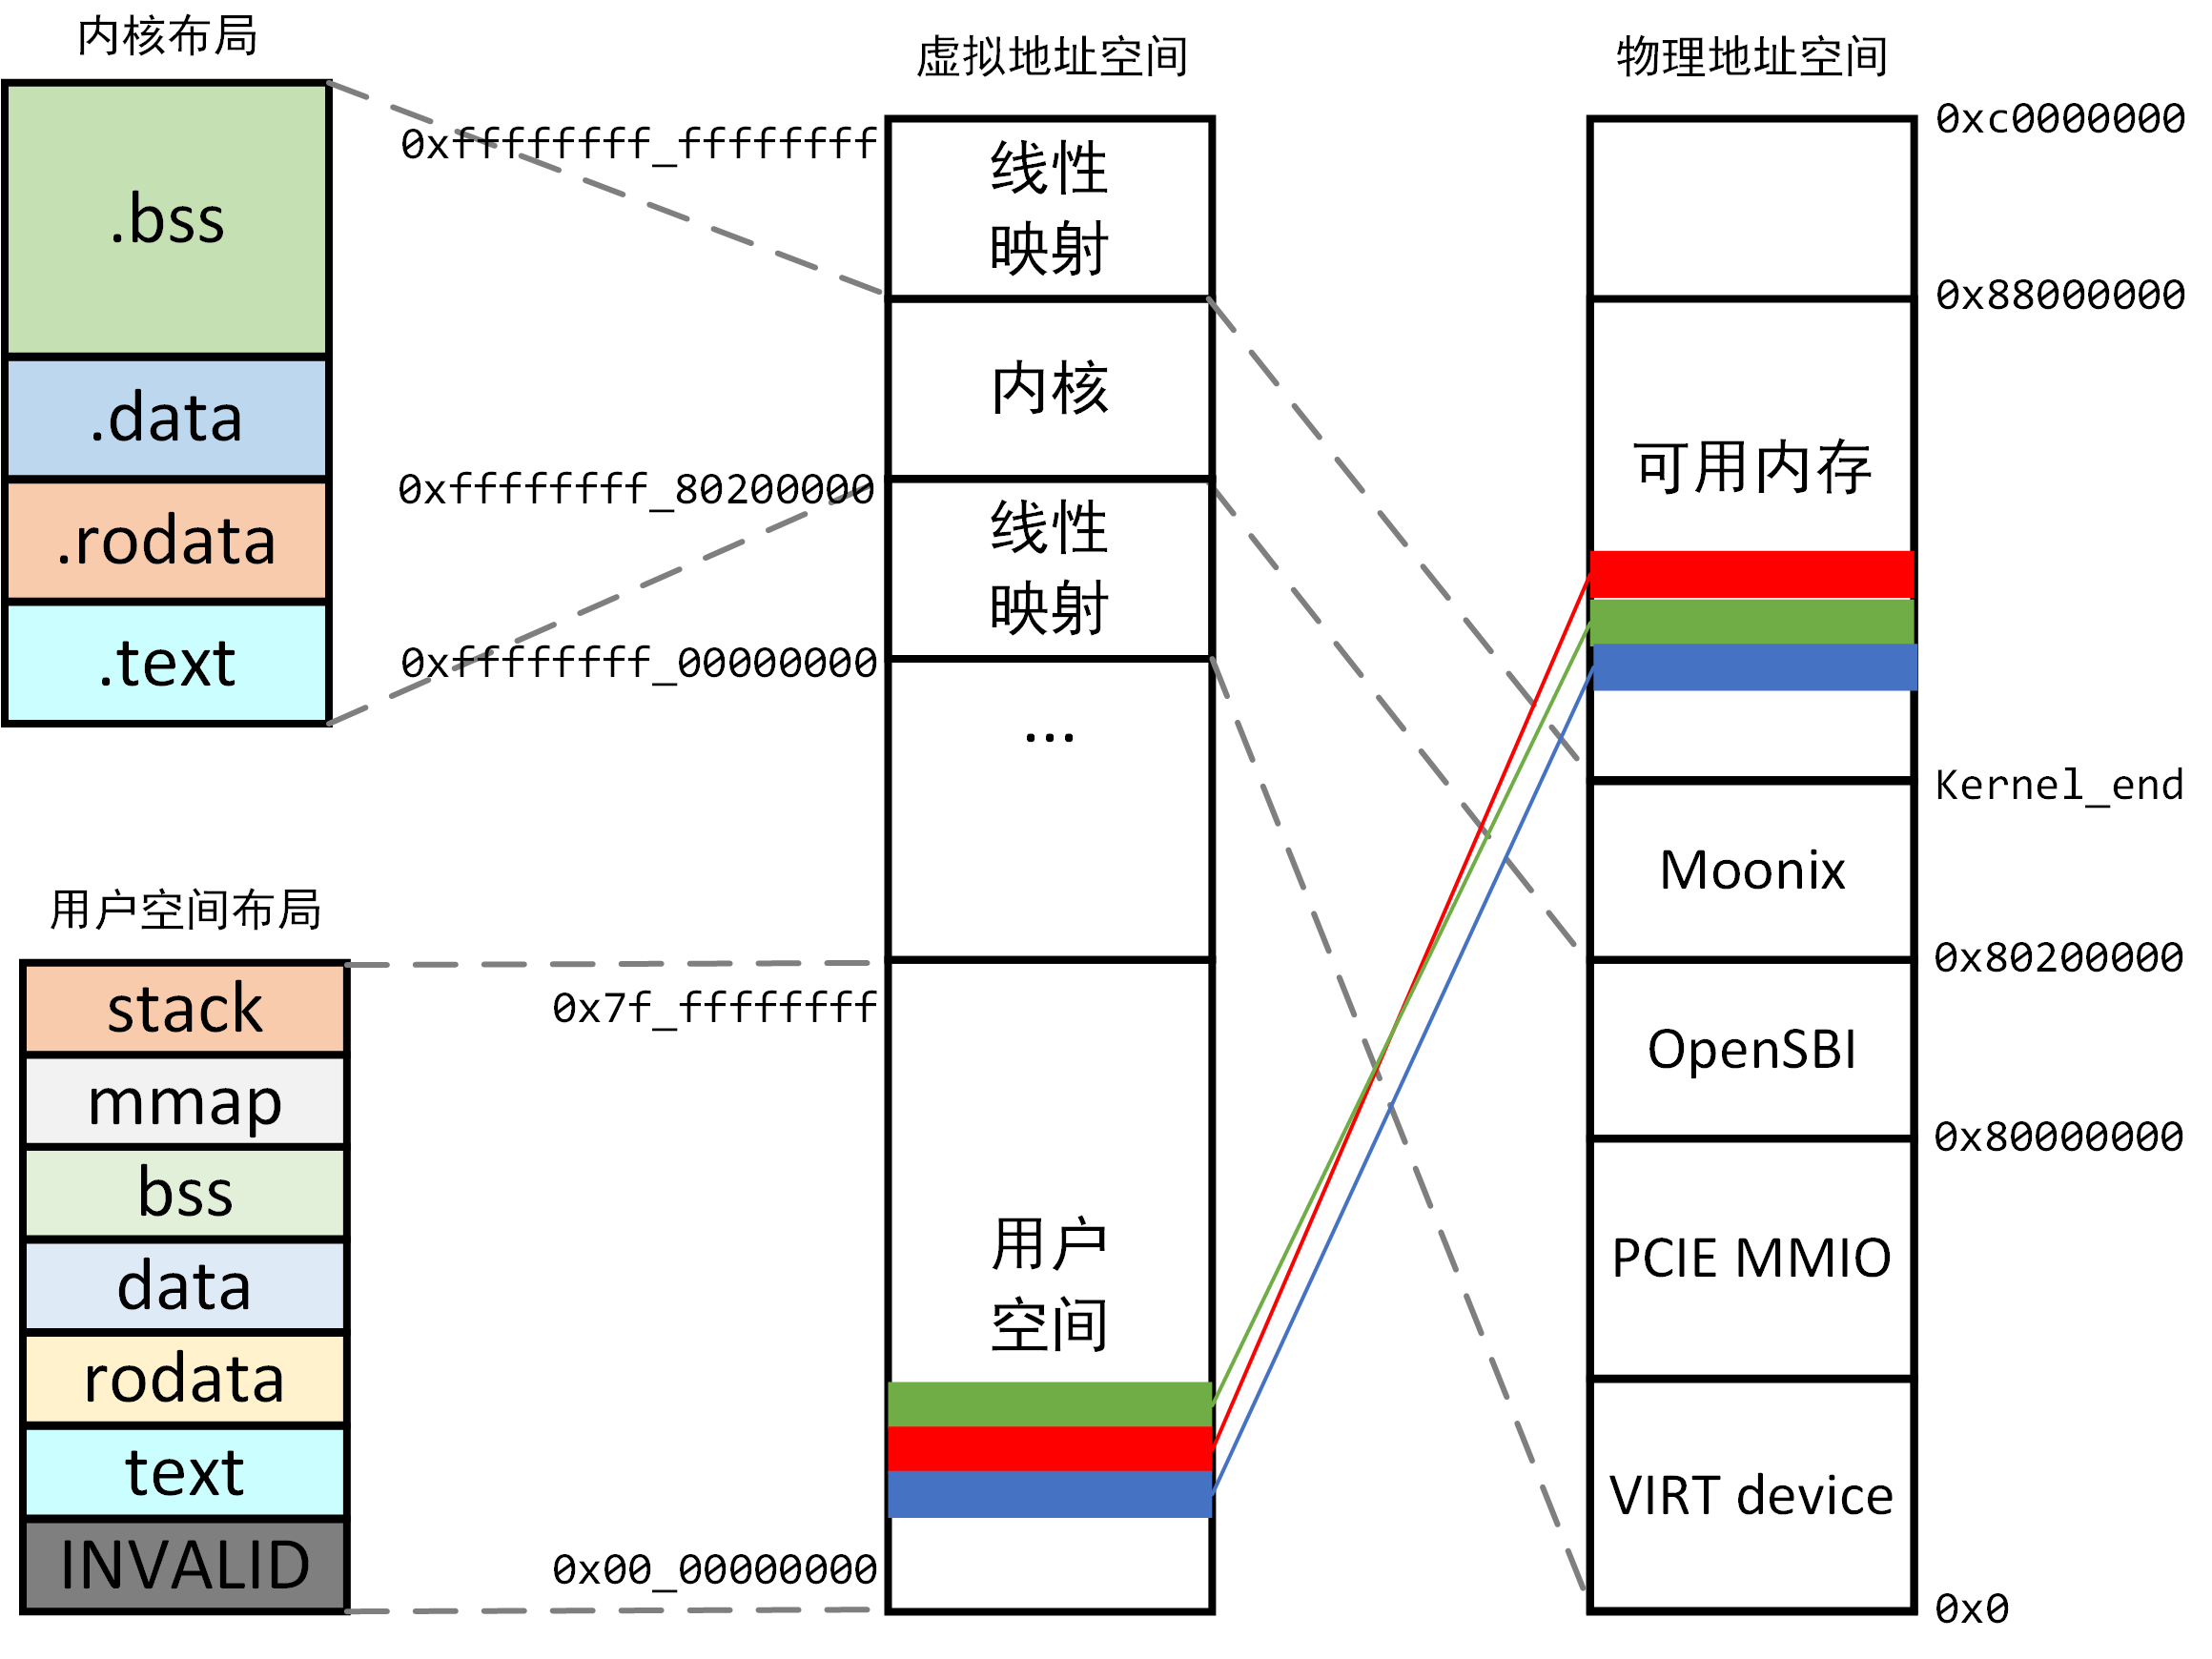
\includegraphics[width=0.55\textwidth]{mem}
	\setlength{\abovecaptionskip}{2pt}
	\caption{Moonix内存结构}
	\label{pic:moonixmem}
\end{figure}

在进程的虚拟地址空间中,进程的私有代码和数据占据了低地址空间,而内核的代码和数据占据了高地址空间。内核需要被映射到每个进程的高地址处,来保证用户进程在发起系统调用陷入内核时,进程能够寻找到内核的处理代码。